\documentclass[12pt]{article}
\usepackage[margin=1in]{geometry}
\geometry{letterpaper}                  
\usepackage{graphicx}
\usepackage[hyphens]{url}
\usepackage{fancyhdr}
\pagestyle{fancy}
\usepackage{fixltx2e}
\usepackage{amsmath,amsfonts,amsthm,amssymb}
\usepackage{graphicx}
\usepackage{algorithm}
\usepackage{algorithmic}
\usepackage{url}
\usepackage[normalem]{ulem}
\usepackage[pdftex]{color}
\usepackage{varioref}
\usepackage{mathrsfs}
\usepackage{amsmath}
\labelformat{equation}{\textup{(#1)}}
\usepackage[sort&compress,colon,square,numbers]{natbib}


\usepackage{color}
\newcommand{\todo}[1]{{\color{red}{\it TODO: #1}}}
\newcommand{\jovo}[1]{{\color{green}{\it jovo: #1}}}
\newcommand{\will}[1]{{\color{blue}{\it will: #1}}}
\newcommand{\greg}[1]{{\color{cyan}{\it greg: #1}}}


\begin{document}

\begin{center}\Large \bf EN.580.694: Statistical Connectomics \\ Final Project \end{center}
\begin{center} Indigo V. L. Rose $\cdot$ \today  \end{center}
\bigskip


\section*{Clustering Algorithms Engineering of the Mouse Neocortex Connectome}

\begin{figure}[h]
\begin{center}
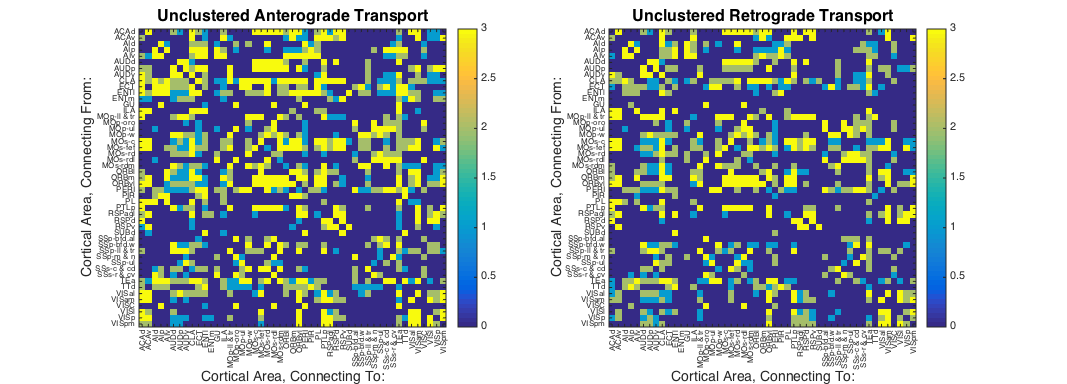
\includegraphics[width=1\textwidth]{figure1}
\caption{The unclustered data from the mouse connectome, identified by [1]. The anterograde and the retrograde tracer data was averaged together to create a combined matrix. Clustering algorithms were performed on these matrix.}
\end{center}
\end{figure}

\paragraph{Opportunity}

Recent advances in increasingly higher resolution axon tracing techniques have enabled the compilation of whole connectomes at an unprecedented level [1]. The Mouse Connectome Project assembled a complete cortico-cortical mesoscale connectome for the mouse cortex, allowing researchers to examine the interconnectivity of the mouse neocortex. The data gleaned from this has far-reaching implications for how the brain communicates and processes information, and is the first step to understanding human cognition from the brain's connectomic architecture [2]. Clustering the data into subnetworks allows for quasi-independent analyses of network systems, showing specialization of areas which can confirm anatomical data or suggest new approaches for how subnetworks support behaviors. 

\paragraph{Challenge}

Identifying subnetworks of the connectome is not a straight-forward task. There are countless algorithms for clustering which each have their pros and cons. It's difficult to compare which nodes form which networks and how they all fit together. This project will examine a few common algorithms and compare them to see what the paper [1] did and what might work better.

\paragraph{Action}

The raw data will need to be copied from Zingg, Hintiryan, et al. and processed into a binary, combined matrix. Two \texttt{kmeans} algorithms were ran, one with k=4 and one with k=12. A major difficulty of \texttt{kmeans} is that it needs the number of clusters \textit{a priori}. Four major subnetworks were identified by [1], each composed of many smaller modules, 12 in total. This is why k=4 and k=12 were chosen. These two clustering algorithms were then compared to in silhouette graphs and sorted bar graphs. Several hierarchical clustering algorithms were also ran. The hierarchical linkage methods used were: "simple", "complete", "average" and "weighted". There are then plotted in dendrograms and compared (Figure 2). Finally, a complete (non-binary) matrix was arranged and plotted (Figure 3).

\begin{figure}[h]
\begin{center}
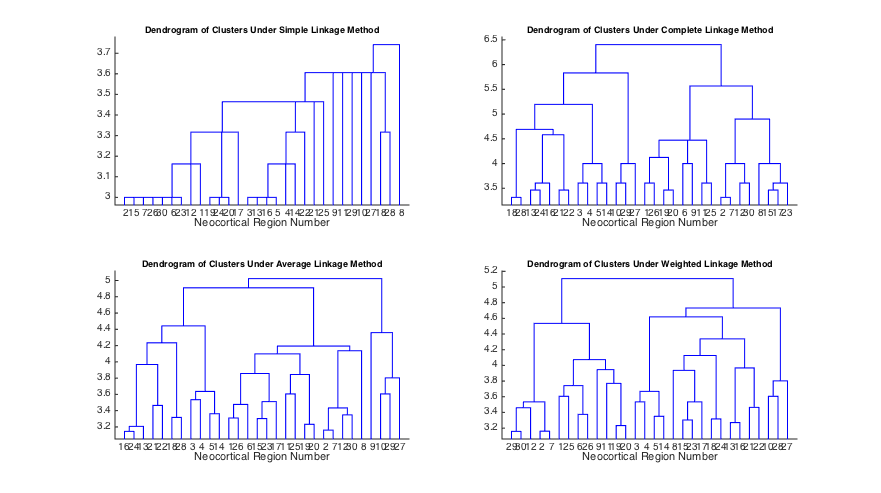
\includegraphics[width=1\textwidth]{figure2} % Include the image placeholder.png
\caption{Four dendrograms for four different hierarchical clustering algorithms.}
\end{center}
\end{figure}

\paragraph{Resolution}

The paper identified 4 major subnetworks (Somatic Sensiomotor, Medial, Lateral, and Claustrum-Entorhinal), many composed of various smaller modules (12 in total). The results from the clustering algorithms show various ways to group the data. Which methods work the best were not analyzed empirically in this paper. However, different algorithms work for different purposes: a hierarchical clustering method makes a lot more sense when looking at how brain systems are related hierarchically, which a more simple \texttt{kmeans} is more useful for identifying larger modules. 

\begin{figure}[h]
\begin{center}
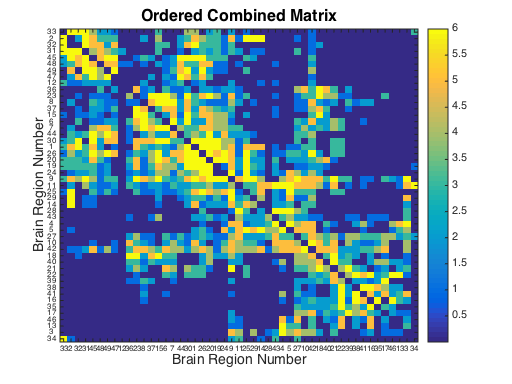
\includegraphics[width=0.7\textwidth]{figure3} % Include the image placeholder.png
\caption{The final compiled matrix, the higher the number the more strong the connection. The brain region number maps to he labels included in the directory where this file lives. }
\end{center}
\end{figure}

\paragraph{Future Work}

The analysis of clustering algorithm used provides a tool to understand the assumptions made by the various algorithms which will allow more careful cognizance of what clustering of nodes means for the mouse neocortex. It's also a starting point to reexamine which clustering method is really the best when dealing with this data of this time and how to implement it in future mesoscale connectomic research. The next step from this paper is to empirically analyze the clustering algorithms and see how they perform to the algorithms used in [1]. 

% \begin{figure}[h]
% \begin{center}
% 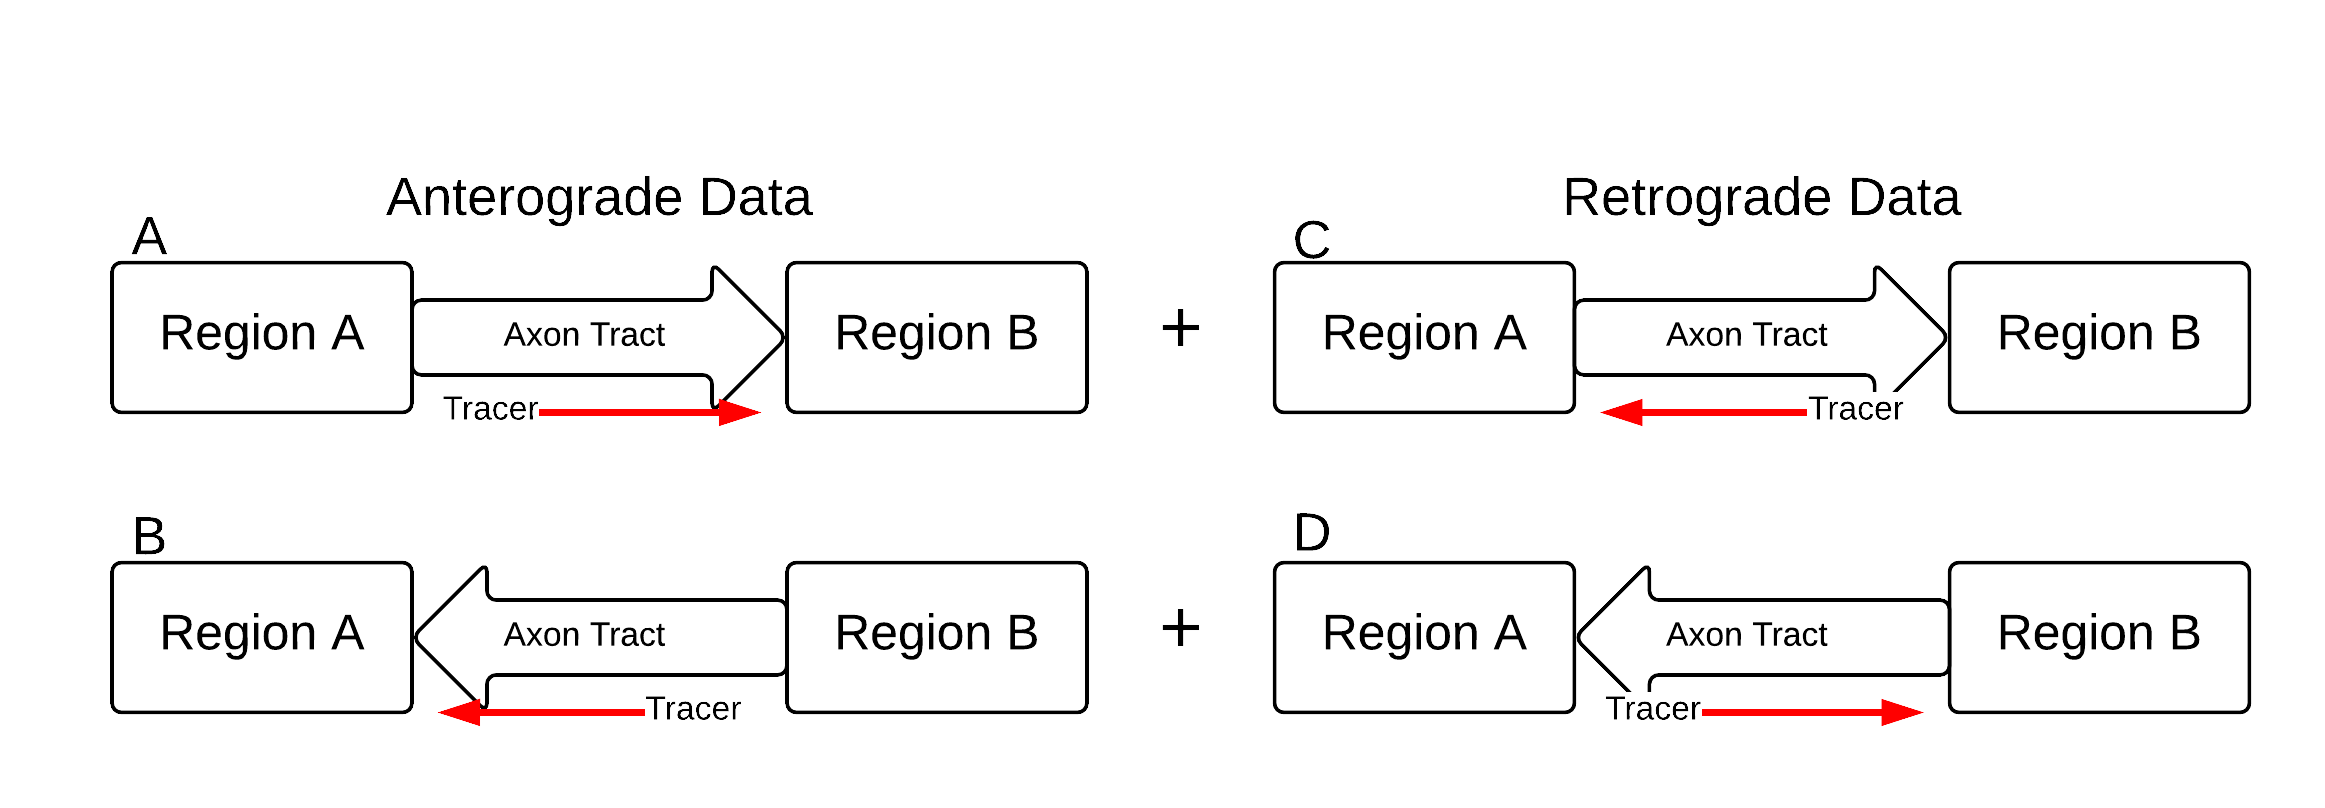
\includegraphics[width=0.6\textwidth]{figure4} % Include the image placeholder.png
% \caption{The method by which the matrix \texttt{cmat\_bin} can be compiled from two matrices, \texttt{ant} and \texttt{ret}, for anterograde and retrograde transport matrices. The data from A and C and averaged together to form one triangle of the compiled matrix. The data from B and D are similarly averaged to form the other triangle of the matrix, \texttt{cmat\_bin}.}
% \end{center}
% \end{figure}


\paragraph{References}

\begin{enumerate}
\item{Brian Zingg, Houri Hintiryan, Lin Gou, Monica�Y. Song, Maxwell Bay, Michael�S. Bienkowski, Nicholas�N. Foster, Seita Yamashita, Ian Bowman, Arthur�W. Toga, Hong-Wei Dong, Neural Networks of the Mouse Neocortex, Cell, Volume 156, Issue 5, 27 February 2014, Pages 1096-1111, ISSN 0092-8674, http://dx.doi.org/10.1016/j.cell.2014.02.023.}

\item{Sporns O, Tononi G, K�tter R (2005) The Human Connectome: A Structural Description of the Human Brain. PLoS Comput Biol 1(4): e42. doi:10.1371/journal.pcbi.0010042.}
\end{enumerate}

\end{document}  